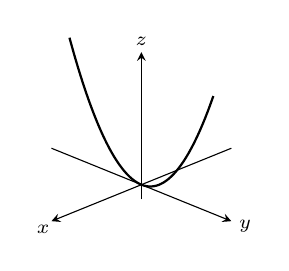
\begin{tikzpicture}[>=stealth]
\begin{axis}%
[width=175pt,tick label style={font=\scriptsize},axis on top,
			axis lines=center,
			view={135}{35},
			name=myplot,
			xtick=\empty,
			ytick=\empty,
			ztick=\empty,
			ymin=-2.5,ymax=2.5,
			xmin=-2.5,xmax=2.5,
			zmin=-.5, zmax=4.5,
			every axis x label/.style={at={(axis cs:\pgfkeysvalueof{/pgfplots/xmax},0,0)},xshift=-3pt,yshift=-3pt},
				xlabel={\scriptsize $x$},
			every axis y label/.style={at={(axis cs:0,\pgfkeysvalueof{/pgfplots/ymax},0)},xshift=5pt,yshift=-2pt},
				ylabel={\scriptsize $y$},
				every axis z label/.style={at={(axis cs:0,0,\pgfkeysvalueof{/pgfplots/zmax})},xshift=0pt,yshift=4pt},
				zlabel={\scriptsize $z$}
			]



\addplot3[domain=-2:2,,thick,smooth,samples y=0,{\colorone},%surf,%fill=white,
samples=30,] ({0},{x},{x^2});


%\foreach \z in {-1.9,-1.6,...,1.9}
%{\addplot3[domain=-2:2,,thick,smooth,samples y=0,{\colortwo},%surf,%fill=white,
%samples=30,] ({x},{\z},{\z*\z});
%}


\end{axis}

\end{tikzpicture}











